% Print
\documentclass[DIV=15,headinclude=true]{scrartcl}

%Packages, die für die deutsche Sprache erforderlich sind
\usepackage[utf8]{inputenc}
\usepackage[T1]{fontenc}
\usepackage{lmodern}
\usepackage[ngerman]{babel}
\usepackage{csquotes}

%Packages für Graphik
\usepackage[]{graphicx}
\graphicspath{{figures/}}

%BibLaTex
\usepackage[backend=biber]{biblatex}
\addbibresource{literature/bibliography.bib} 

%Package, damit Bibtex-URL klappt
\usepackage[pdfusetitle]{hyperref}
\usepackage{url}

%Noch schönere Typographie
\usepackage{microtype}

%Kästen
\usepackage{framed}

%Package für schöne Tabellen mit variabler Breite
%\usepackage{tabularx}
\usepackage{tabulary}
\usepackage{booktabs}

%%%%% BEGINN KOPF- UND FUẞZEILE %%%%%
\usepackage[headsepline,footsepline]{scrlayer-scrpage}
\usepackage{graphicx}
\pagestyle{scrheadings}
\ohead{\includegraphics[height=1cm]{figures/bluemarble}}
\chead{\headmark}
\automark{section}
%\ihead{\includegraphics[height=1cm]{bluemarble.jpg}}
\ifoot{\csname @title\endcsname}\cfoot{\pagemark}
\ofoot{\today}
%%%%% ENDE KOPF- UND FUẞZEILE %%%%%

\begin{document}
%%%%% BEGINN TITEL %%%%%
\title{Prüfungsleistungen und Bewertungskriterien}
\subtitle{Entwicklungsmethoden Nachhaltiger Produkte}
\author{EnWiNaP-Team}
\maketitle
%%%%% ENDE TITEL %%%%%

%%%%% BEGINN FRONT MATTER %%%%%
\tableofcontents
%%%%% ENDE FRONT MATTER %%%%%


%%%%% BEGINN INHALT %%%%%
\section{Über dieses Dokument}

Wir wollen hier unsere Gedanken zur Bewertung zusammenfassen und
transparent mit allen Beteiligten konzipieren. Das Dokument ist als
\enquote{lebendiges Dokument} konzipiert, das im Laufe der ersten
Durchführung (und danach -- aber langsamer) weiterentwickelt wird. Die
Entwicklung geschieht auf GitLab unter
\href{https://github.com/mpm-tu-berlin/lehre-enwinap}{\texttt{https://github.com/mpm-tu-berlin/lehre-enwinap}}

\section{Prüfungsleistungen}

\begin{table}\centering
	\label{tab:zusammensetzung}
	\caption{Zusammensetzung der Gesamtnote}
	\begin{tabular}{llr}
		\toprule
		Name           & Typ         & Gewichtung \\
		\midrule
		Name           & Typ         & Gewichtung \\
		Lernjournal    & individuell & 40 \%      \\
		Präsentation   & Gruppe      & 20 \%      \\
		Projektbericht & Gruppe      & 40 \%      \\
		\bottomrule
	\end{tabular}
\end{table}

Die Veranstaltung ist als Portfolioprüfung\footnote{Rahmenbedingungen:
	\href{https://www.tu-berlin.de/asv/menue/gremien/kommissionen_des_as/hinweise_zur_allgstupo/hinweise_zu_portfoliopruefungen/}{\underline{hier}}}
konzipiert. Tabelle \ref{tab:zusammensetzung} zeigt die
Zusammensetzung der Gesamtnote auf die einzelnen Teilleistungen.

\begin{table}\centering
	\label{tab:notenschluessel}
	\caption{Notenschlüssel}
	\begin{tabular}{lr}
		\toprule
		Punktzahl   & Note \\
		\midrule
		Punktzahl   & Note \\
		\(\geq\) 85 & 1,0  \\
		\(\geq\) 80 & 1,3  \\
		\(\geq\) 75 & 1,7  \\
		\(\geq\) 70 & 2,0  \\
		\(\geq\) 65 & 2,3  \\
		\(\geq\) 60 & 2,7  \\
		\(\geq\) 55 & 3,0  \\
		\(\geq\) 50 & 3,3  \\
		\(\geq\) 45 & 3,7  \\
		\(\geq\) 40 & 4,0  \\
		\(<\) 40    & 5,0  \\
		\bottomrule
	\end{tabular}
\end{table}

Zur Zuordnung der Portfoliopunkte zu den Noten kommt der
\enquote{Notenschlüssel 3} der Fakultät IV zur Anwendung, wie in Tabelle
\ref{tab:notenschluessel} gezeigt. Dieser
Notenschlüssel ist \enquote{großzügiger} als die üblicherweise an der
Fakultät V verwendeten. Wir wollen eine Lehrveranstaltung, in der
\enquote{sehr gut} nicht \enquote{fehlerfrei} bedeuten muss und wir
nicht eine Korrektur für die Punkte machen und eine, in der wir alle
Fehler aufzählen, die uns zwar aufgefallen sind aber für die wir keine
Punkte abziehen können, weil sonst die Note zu schlecht wird.
Studierende sollten also damit rechnen, das die Punktzahlen der
Teilleistungen schlechter als gewohnt ausfallen, die Noten jedoch nicht.

\subsection{Lernjournal}

\subsubsection{Beschreibung}

\emph{Ziel} des Lernjournals ist es, sich mit den vermittelten Inhalten
selbstständig erneut auseinanderzusetzen und sie in einem sorgfältig
erstellten Dokument aufzubereiten. Neben der Reproduktion sollen hier
auch eigene Einschätzungen und Interpretationen der Inhalte vermerkt
werden.

\emph{Formell} werden keine umfangreichen Anforderungen gestellt. Eine
\enquote{wissenschaftliche} Form (z.~B. so wie dieses Dokument +
Quellen) ist genauso akzeptabel wie eine kreativere Auseinandersetzung
mit Mindmaps, Zeichnungen und viel buntem Papier. Die Abgabe kann
physisch oder elektronisch erfolgen.

Wir erwarten einen \emph{Umfang} von ein bis zwei A4-Seiten (oder dem
Äquivalent dazu in anderen Formaten) für jeden Themenblock.

\subsubsection{Bewertungskriterien}

Unten einige Grundlegende Gedanken, die exakte Bepunktung ist in
Abbildung \protect\hyperlink{abb:lernjournal}{1} zu sehen.

\begin{description}
	\item[Selbstständigkeit]
	      Die Aufgabe sollte jede Studentin selbstständig ohne fremde Hilfe
	      durchführen.
	\item[Vollständigkeit]
	      Wir erwarten, dass jeder Themenblock bearbeitet wird. Das bedeuted
	      nicht, dass die Studierenden den gesamten Inhalt der Themenblöcke
	      reproduzieren sollen, sondern, dass sie sich mit jedem Themenblock
	      auseinander setzen und diesen reflektieren sollen.
	\item[Inhalt]
	      Wir möchten einen oder mehrere Kerninhalte unserer Themenblöcke (oder
	      dass, was die Studierenden als Kerninhalte wahrnehmen) wiedererkennen.
	      Wie im Bereich \emph{Vollständigkeit} hervorgehoben, sollen die Inhalte
	      der Themenblöcke reflektiert werden, die Studierenden sollen sich in
	      einer selbstgewählten Form mit den behandelten Themenblöcken auseinander
	      setzen. Das bietet die Möglichkeit, sich beispielsweise sehr detailliert
	      mit einer Kernthematik auseinander zu setzen oder die gesamten
	      Kerninhalte hollistisch zu betrachten oder einen Weg dazwischen zu
	      wählen. Dies ist den Studierenden freigestellt.
	\item[Struktur]
	      Die Inhalte sollten sinnvoll Anhand des \emph{Inhalts} strukturiert und
	      kategorisiert sein, nicht bloß so, wie die Vorlesung ablief.
	\item[Eigene Gedanken]
	      War es für euch neu oder schon bekannt? War es logisch schlüssig oder
	      unerwartet? Glaubt ihr, das die Inhalte des Themenblockes so stimmen,
	      oder kritisiert ihr unsere Meinungen und Fakten?
	\item[Form]
	      Das Lernjournal sollte frei von Rechtschreib-, Grammatik- und
	      Zeichenfehlern und (ungewollten) Stilbrüchen sein.
\end{description}

\begin{figure}
	\centering
	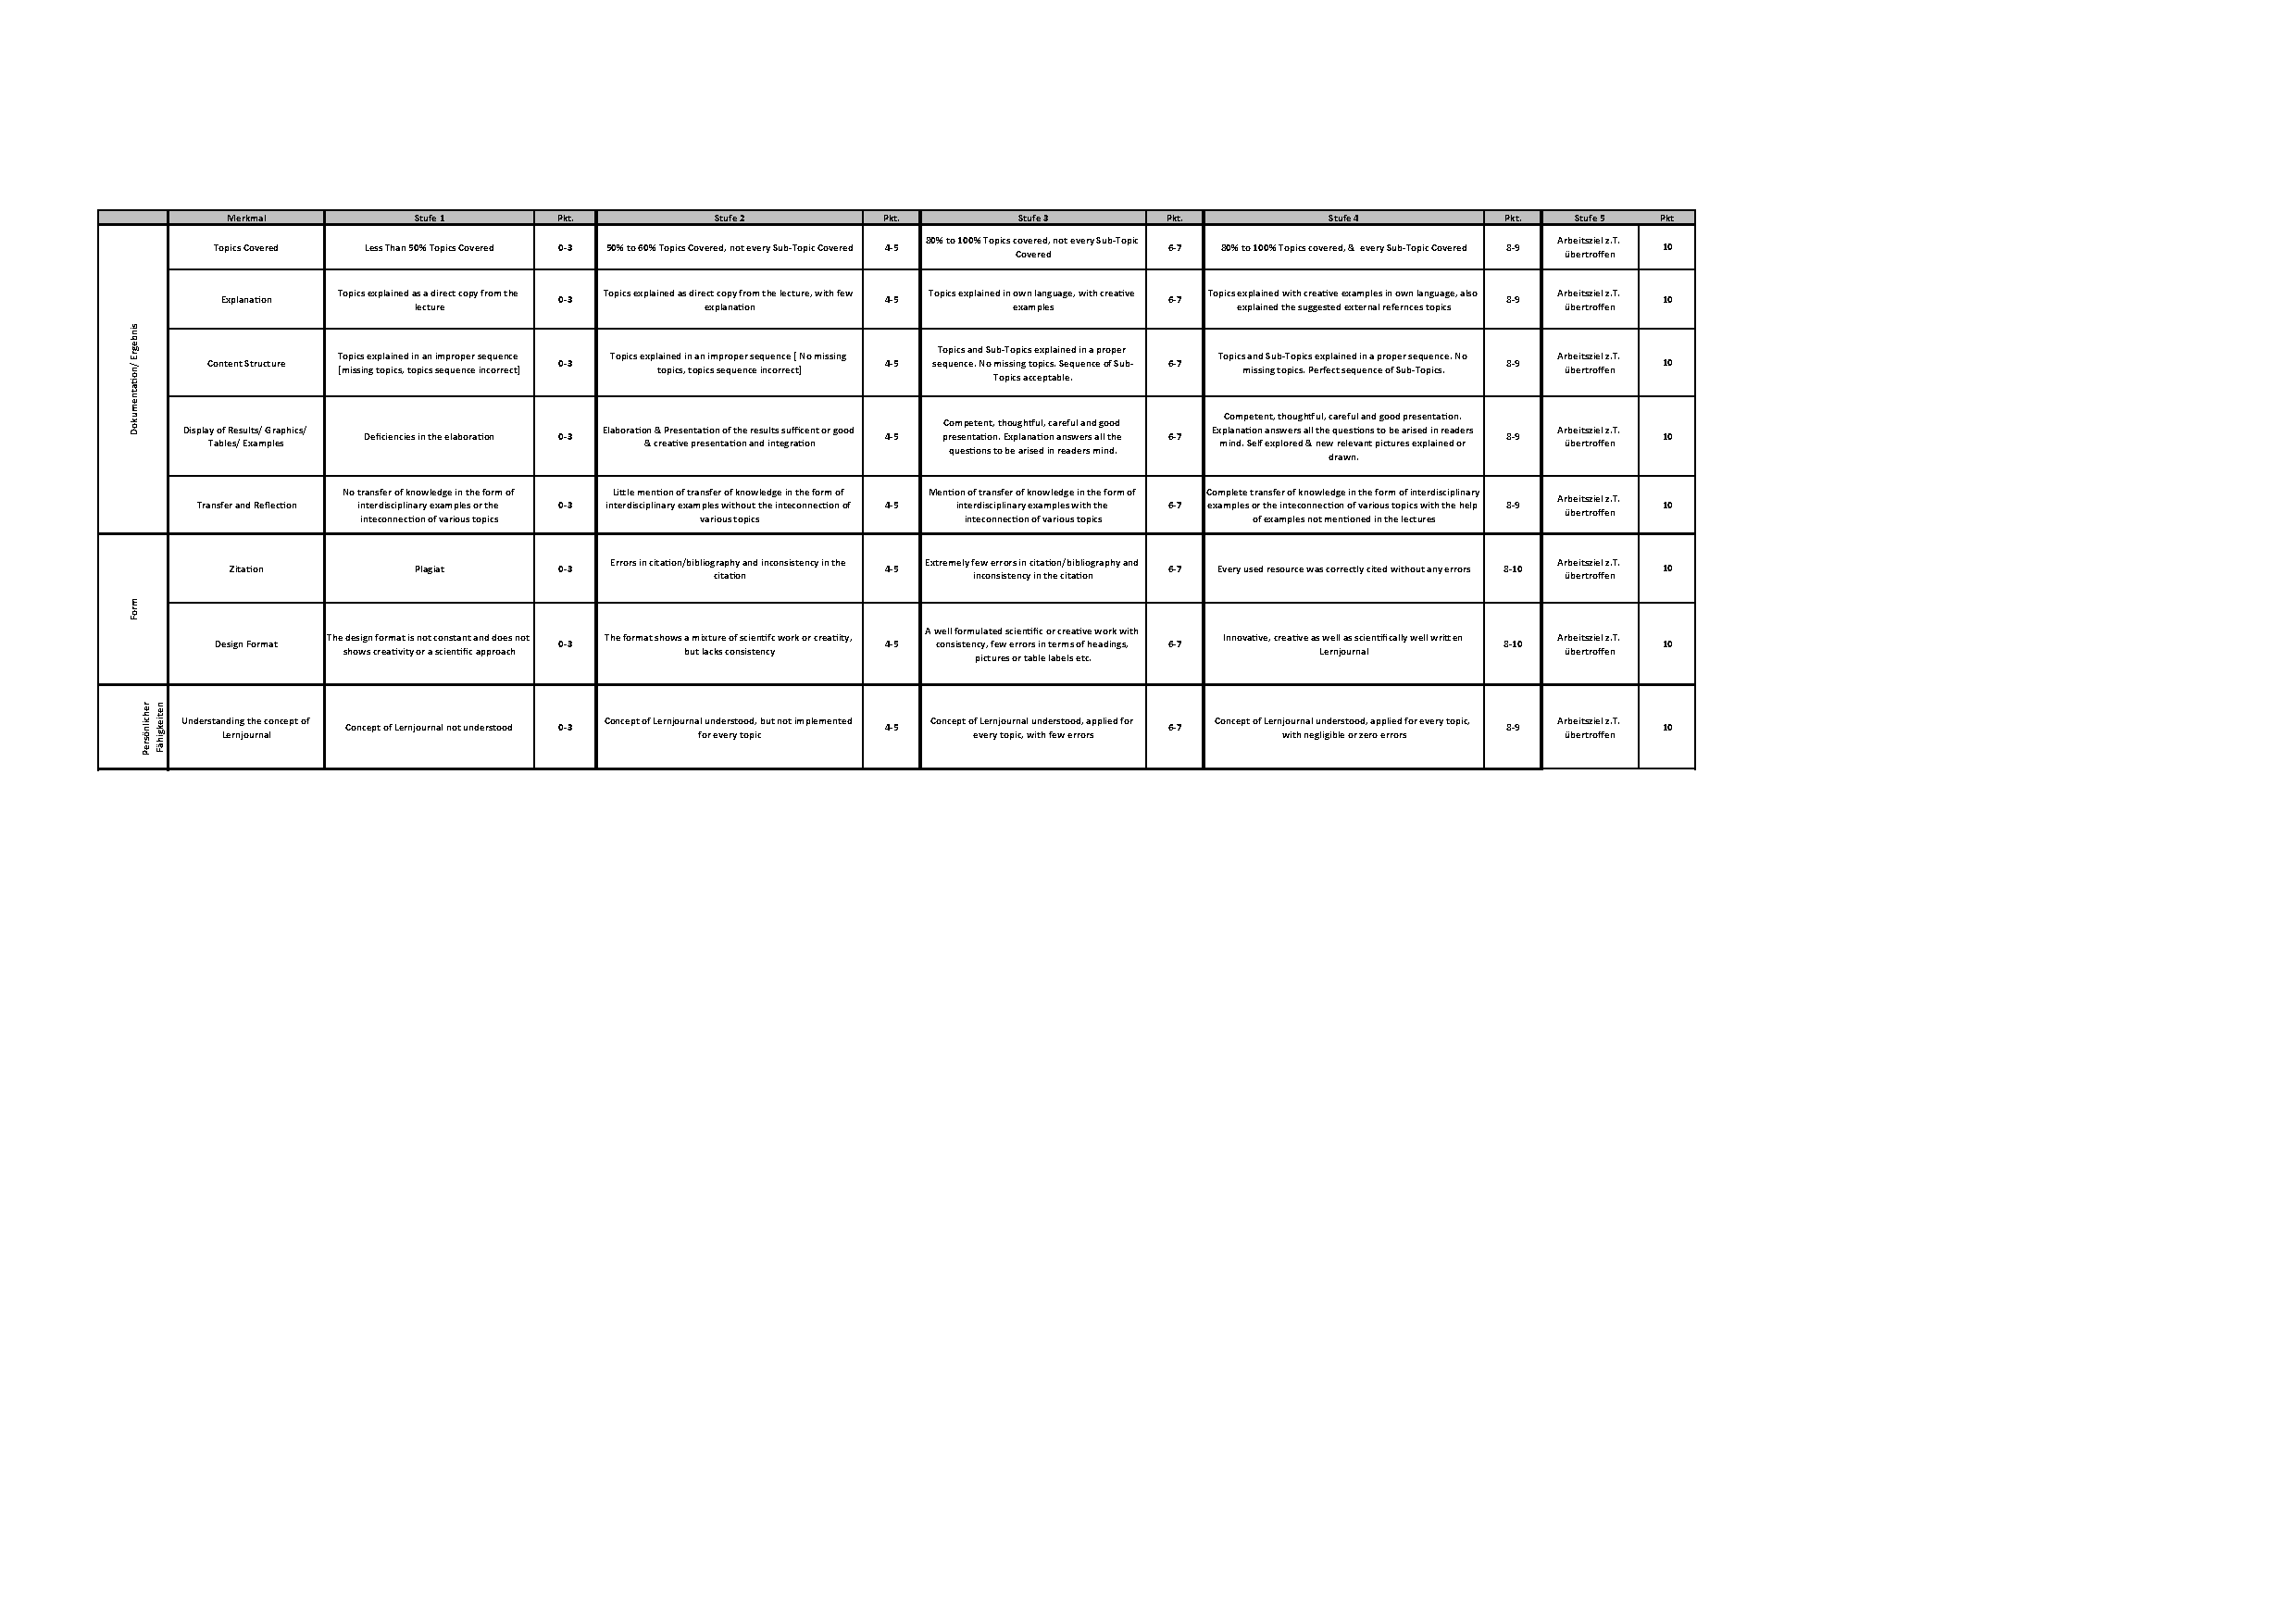
\includegraphics[width=\textwidth]{figures/lernjournal}
	\caption{Bewertungskriterien Lernjournal}
	\label{abb:lernjournal}
\end{figure}

\subsection{Präsentation}

\subsubsection{Beschreibung}

\emph{Ziel} der Präsentation ist es, eure Ergebnisse zu einer
Teilaufgabe des Projektes mit euren Kolleginnen zu teilen und eine
Diskussion darüber zu führen. Es soll \emph{nicht} um eine bloße -- am
schlimmsten noch bei allen Gruppen gleiche -- Projektpräsentation gehen,
sondern um die Gestaltung einer Mini-Lehreinheit zu einem bestimmten
Thema.

\emph{Formell} wird ein Zeitrahmen von 30 Minuten und eine
Wissensvermittlung und Diskussion mit allen Teilnehmern gefordert.
Voraussichtlich muss die Präsentation online stattfinden. Weitere
Anforderungen (Medium, Software, Redeanteile) gibt es nicht.

\subsubsection{Bewertungskriterien}

\begin{framed}

	\emph{Bewertungskriterien Präsentation -- orientieren an bisherigen
		Präsentationen am Fachgebiet MPM, aber
		Interaktivität/Diskussionsgestaltung einbeziehen}

\end{framed}

\subsection{Projektbericht}

\subsubsection{Beschreibung}

\emph{Ziel} des Projektberichts ist es, das gelernte Wissen der
jeweiligen Blöcke anhand von gegebenen Aufgaben auf ein ausgewähltes
Produkt\footnote{Im ersten Durchlauf zur besseren Vergleichbarkeit bei
	allen Gruppen identisch. Später wollen wir auch mal verschiedene
	Produkte ausprobieren.} anzuwenden.

\emph{Formell} gelten die üblichen Ansprüche an eine wissenschaftliche
Arbeit an unserem Fachgebiet, also insbesondere Richtigkeit,
Nachvollziehbarkeit und eine dem Inhalt angemessene Gliederung. Eine
korrekte Zitierweise gehört auch dazu. Das ist fundamental die
Verwendung möglichst hochwertiger Quellen für nicht eigene oder
grundlegende Erkenntnisse und ein Quellenverzeichnis, mit dem man sie
finden kann.

\subsubsection{Bewertungskriterien}

\begin{framed}

	\emph{Bewertungskriterien Projektbericht -- orientieren an
		\enquote{Methodisches Konstruieren} und \enquote{Electric Vehicle
			Technologies and Applications}}

\end{framed}

%%%%% ENDE INHALT %%%%%
\end{document}
